\subsection{Centralized approach}
Figure \ref{fig:cen_power} shows the power profile of the PEVs in the centralized approach. The aggregated power tracks almost perfectly the reference value, without ever exceeding the constraint on the maximum power.
\begin{figure}[H]
    \centering
    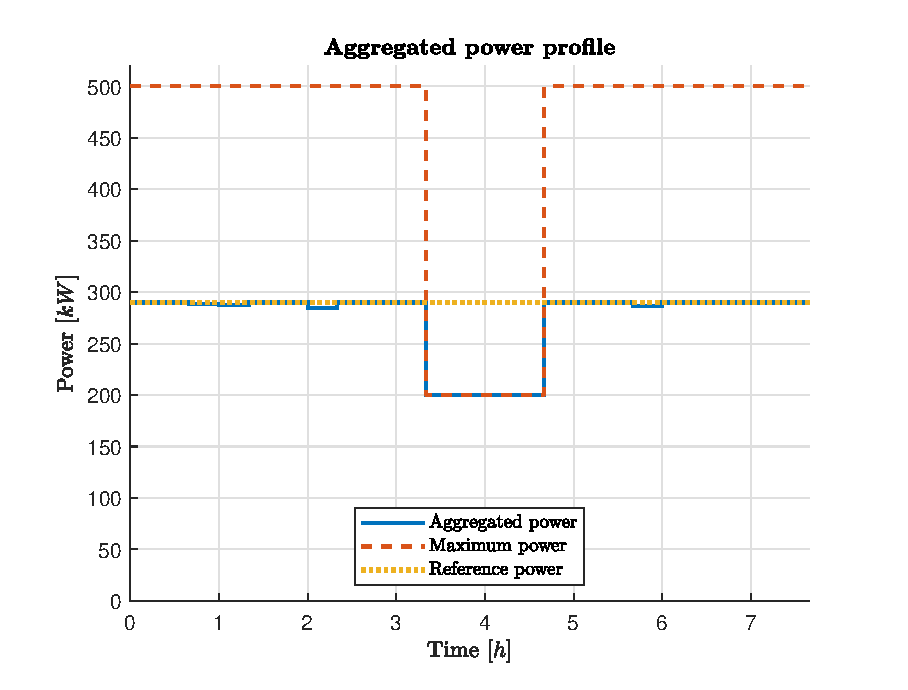
\includegraphics[width=\columnwidth]{figures/images/cen_power.eps}
    \caption{Aggregated power profile of the PEVs in the centralized case.}
    \label{fig:cen_power}
\end{figure}

The state of charge evolution of a random batch of 10 PEVs can be seen in Figure \ref{fig:cen_state}. The state of charge is kept within the limits and the final values reflect the desired ones.
\begin{figure}[H]
    \centering
    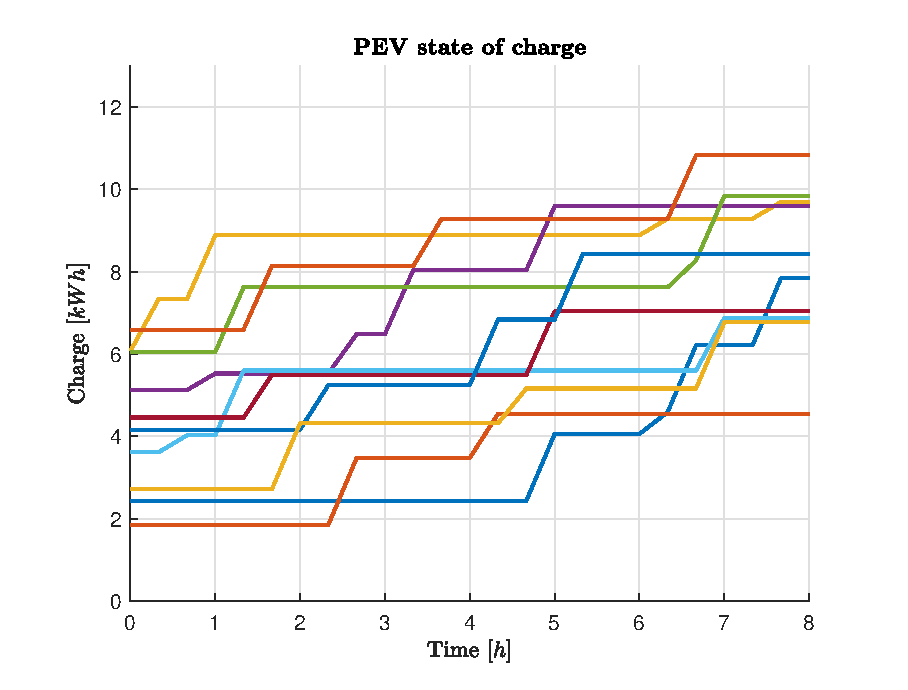
\includegraphics[width=\columnwidth]{figures/images/cen_state.eps}
    \caption{State of charge evolution of the PEVs in the centralized case.}
    \label{fig:cen_state}
\end{figure}

Finding the optimal solution of the centralized problem takes about $414.3\,s \simeq 7\,min $. This is typically not acceptable in a real-world scenario, where the optimization problem should be solved in a significantly shorter time than the duration of the sampling step.